% Multiple Choice Question 35

\begin{center}
    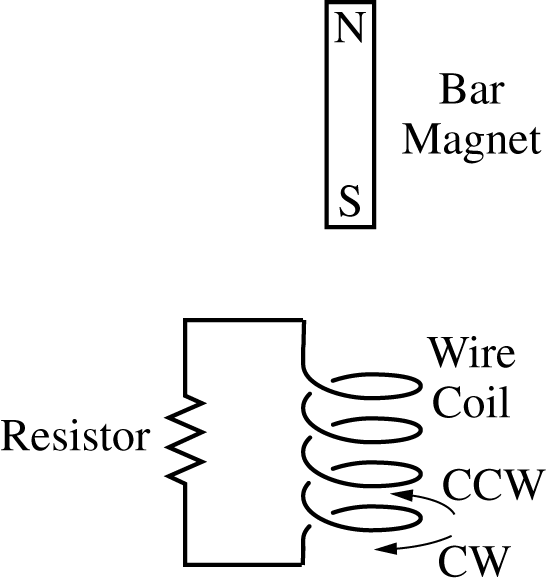
\includegraphics[scale=0.3]{images/img-016-033.png}
\end{center}

\begin{questions}\setcounter{question}{34}\question
A bar magnet with its south pole pointing down is released from rest and falls through a wire coil, as shown above. A resistor is connected across the two ends of the coil. What current would be produced in the coil, as observed by a person directly above the coil?

\begin{choices}
    \choice A clockwise current only
    \choice A counterclockwise current only
    \choice A current that is first clockwise and then counterclockwise
    \choice A current that is first counterclockwise and then clockwise
    \choice No current would be produced.
\end{choices}
\end{questions}
